\chapter{Pengujian Sistem}

Pada pengujian performa akselerator \ac{RL}, terdapat tiga komponen yang penting yang perlu ditinjau:

\begin{enumerate}
	\item Akurasi algoritma dan akselerator perangkat keras.
	\item Utilisasi sumber daya pada akselerator.
	\item Kecepatan akselerator dibanding dengan implementasi perangkat lunak.
\end{enumerate}

Ketiga komponen tersebut, akan diuji dan dibahas hasilnya pada bab ini. Akurasi algoritma akan ditinjau terhadap implementasi \ac{DFS}, begitu pula dengan akselerator. Kecepatan yang akan ditinjau adalah kecepatan pada tahap pembelajaran dan kecepatan pada tahap \textit{inference}. Pengujian kecepatan pada kedua tahap ini dilakukan menggunakan modul \textit{timer} yang dapat menghasilkan perbedaan \textit{clock cycles} dari hasil komputasi pada \textit{processor} VeeR EL2. Implementasi timer yang dibangun pada \textit{processor} VeeR EL2 merupakan adopsi dari spesifikasi OpenCores yang tersedia secara terbuka pada \parencite{open2024ptc}.

\begin{enumerate}
	\item Pembelajaran \acl{RL}\\
	      Pengujian ini akan mencoba membandingkan algoritma \ref{alg:rl-qmemo} yang menggunakan perangkat lunak terhadap algoritma \ref{alg:hw-sw-sep} yang menggunakan akselerator perangkat keras. Keduanya akan diuji pada \textit{processor} yang sama yaitu VeeR EL3.
	\item \textit{Inference} \acl{RL}\\
	      Pengujian ini akan mencoba membandingkan proses pemilihan aksi $a_{max}$ menggunakan metode eksploitasi. Perbandingan dilakukan dari perangkat lunak terhadap akselerator perangkat keras dengan instruksi q.max.
\end{enumerate}

Pada perbandingan performa \textit{inference}, hasil perbedaan waktu delay yang dibutuhkan oleh perangkat lunak dan akselerator akan diekstrapolasi untuk kasus \textit{cart pole balancing} dari sub-bab \ref{sec:rl-kontrol}. Tujuan akhirnya adalah agar dapat memperlihatkan dampak penggunaan akselerator pada suatu kasus fisis yang memerlukan kontrol secara \textit{real time}.

Pada pengujian tersebut, lingkungan pengujian permasalahan \textit{cart pole balancing} dilakukan menggunakan OpenAI Gymnasium \parencite{towers2023gymnasium}. Pada lingkungan OpenAI Gymnasium, permasalahan \textit{cart pole balancing} memiliki spesifikasi pada tabel \ref{tab:state-space-cart-pole}.

\begin{table}[h!]
	\caption{Spesifikasi $State$ untuk \textit{Cart Pole Balancing} dari OpenAI Gymnasium}
	\label{tab:state-space-cart-pole}
	\centering
	\begin{tabular}{|c|c|c|}
		\hline
		Observation           & Min                             & Max                           \\
		\hline
		Cart Position         & -4,8                            & 4,8                           \\
		\hline
		Cart Velocity         & $-\infty$                       & $\infty$                      \\
		\hline
		Pole Angle            & $\sim -0,418$ rad $(-24^\circ)$ & $\sim 0,418$ rad $(24^\circ)$ \\
		\hline
		Pole Angular Velocity & $-\infty$                       & $\infty$                      \\
		\hline
	\end{tabular}
\end{table}

Dengan spesifikasi $state$ sesuai dengan tabel \ref{tab:state-space-cart-pole}, permasalahan \textit{cart pole balancing} dari OpenAI Gymnasium memiliki aksi diskrit sebuah gaya $F$ dengan nilai yang fix, dengan pilihan pemberian gaya ke arah kiri atau kanan. Gambar \ref{fig:cartpole-openai} merupakan ilustrasi yang diberikan oleh OpenAI Gymnasium untuk lingkungan permasalahan \textit{cart pole balancing}.

\begin{figure}[h]
	\centering
	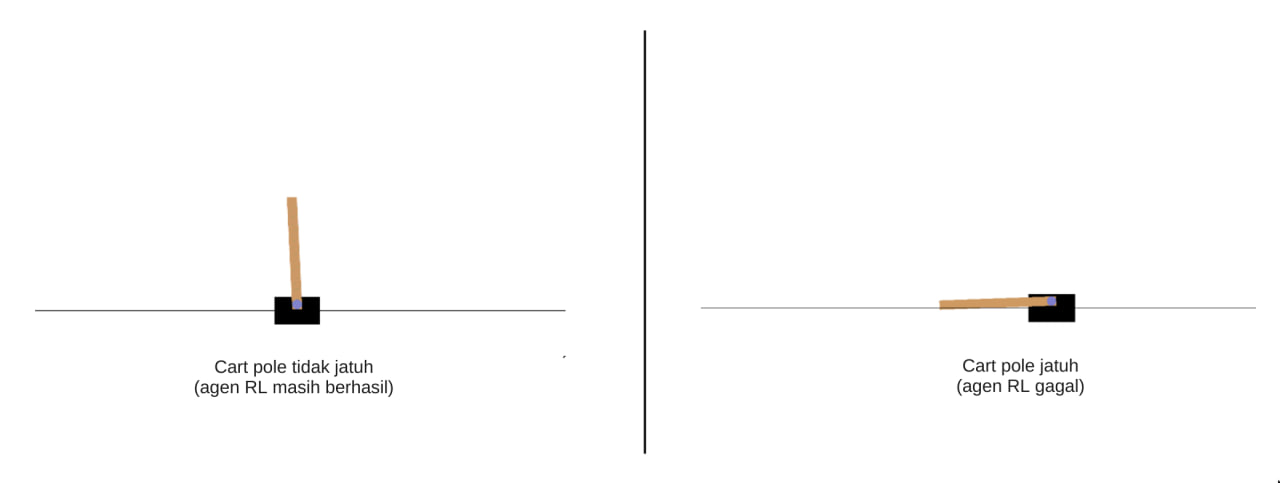
\includegraphics[width=1\textwidth]{chapter-3/cart-pole-openai.jpg}
	\caption{Ilustrasi lingkungan permasalahan \textit{cart pole balancing} OpenAI}
	\label{fig:cartpole-openai}
\end{figure}

Tujuan dari lingkungan permasalahan pada gambar \ref{fig:cartpole-openai} adalah agar terbentukan sebuah model agen \ac{RL} yang mampu menentukan arah gaya yang sesuai untuk setiap saat sehingga \textit{cart pole} tidak jatuh. Tentunya, delay dari komputasi akan sangatlah berpengaruh kepada pengambilan keputusan oleh agen \ac{RL}. Pada permasalahan di penelitian ini, aksi diskrit yang digunakan akan dibuat lebih besar, tidak hanya dua kemungkinan. Kemungkinan dari aksi diskrit akan diperpanjang dengan sebuah limit [$-F$, $F$] dengan pencacahan diskrit sehingga aksi menjadi sebanyak 1.000 kemungkinan. Hal ini dilakukan untuk meninjau kemampuan akselerator untuk mengatasi permasalahan \textit{large branching factor} \parencite{amado2018qtable}.

\section{Akurasi Akselerator}

\section{Utilisasi Sumber Daya Akselerator}

Pada subbab \ref{sec:fpga}, metrik utilisasi sumber daya terdiri atas 3 hal:

\begin{enumerate}
	\item \acf{LUTs}\\
	      \ac{LUTs} adalah blok dasar dari logika yang digunakan dalam \ac{FPGA}. Metrik penggunaan \ac{LUTs} mengindikasikan seberapa banyak sumber daya logika yang digunakan oleh desain pada \ac{FPGA}. Semakin tinggi penggunaan \ac{LUTs}, semakin kompleks dan padat logika yang diimplementasikan.
	\item \textit{Flip-flops}\\
	      \textit{Flip-flops} adalah elemen penyimpanan dasar dalam \ac{FPGA} yang digunakan untuk menyimpan bit data. Penggunaan \textit{flip-flops} mencerminkan kebutuhan desain terhadap penyimpanan data sementara dan kemampuan untuk menangani operasi sekuensial.
	\item \textit{Block \ac{RAM}}\\
	      \textit{Block \ac{RAM}} adalah memori terintegrasi dalam \ac{FPGA} yang digunakan untuk menyimpan data dalam jumlah besar. Metrik penggunaan \textit{block \ac{RAM}} memberikan gambaran tentang kebutuhan desain terhadap memori, termasuk berapa banyak data yang perlu disimpan dan diakses secara cepat selama operasi.
\end{enumerate}

Berikut, pada gambar \ref{fig:plot-resource}, merupakan hasil utilisasi sumber daya akselerator dari sintesis desain \textit{processor} VeeR EL2 tanpa dan dengan implementasi akselerator.

\begin{figure}[h]
	\centering
	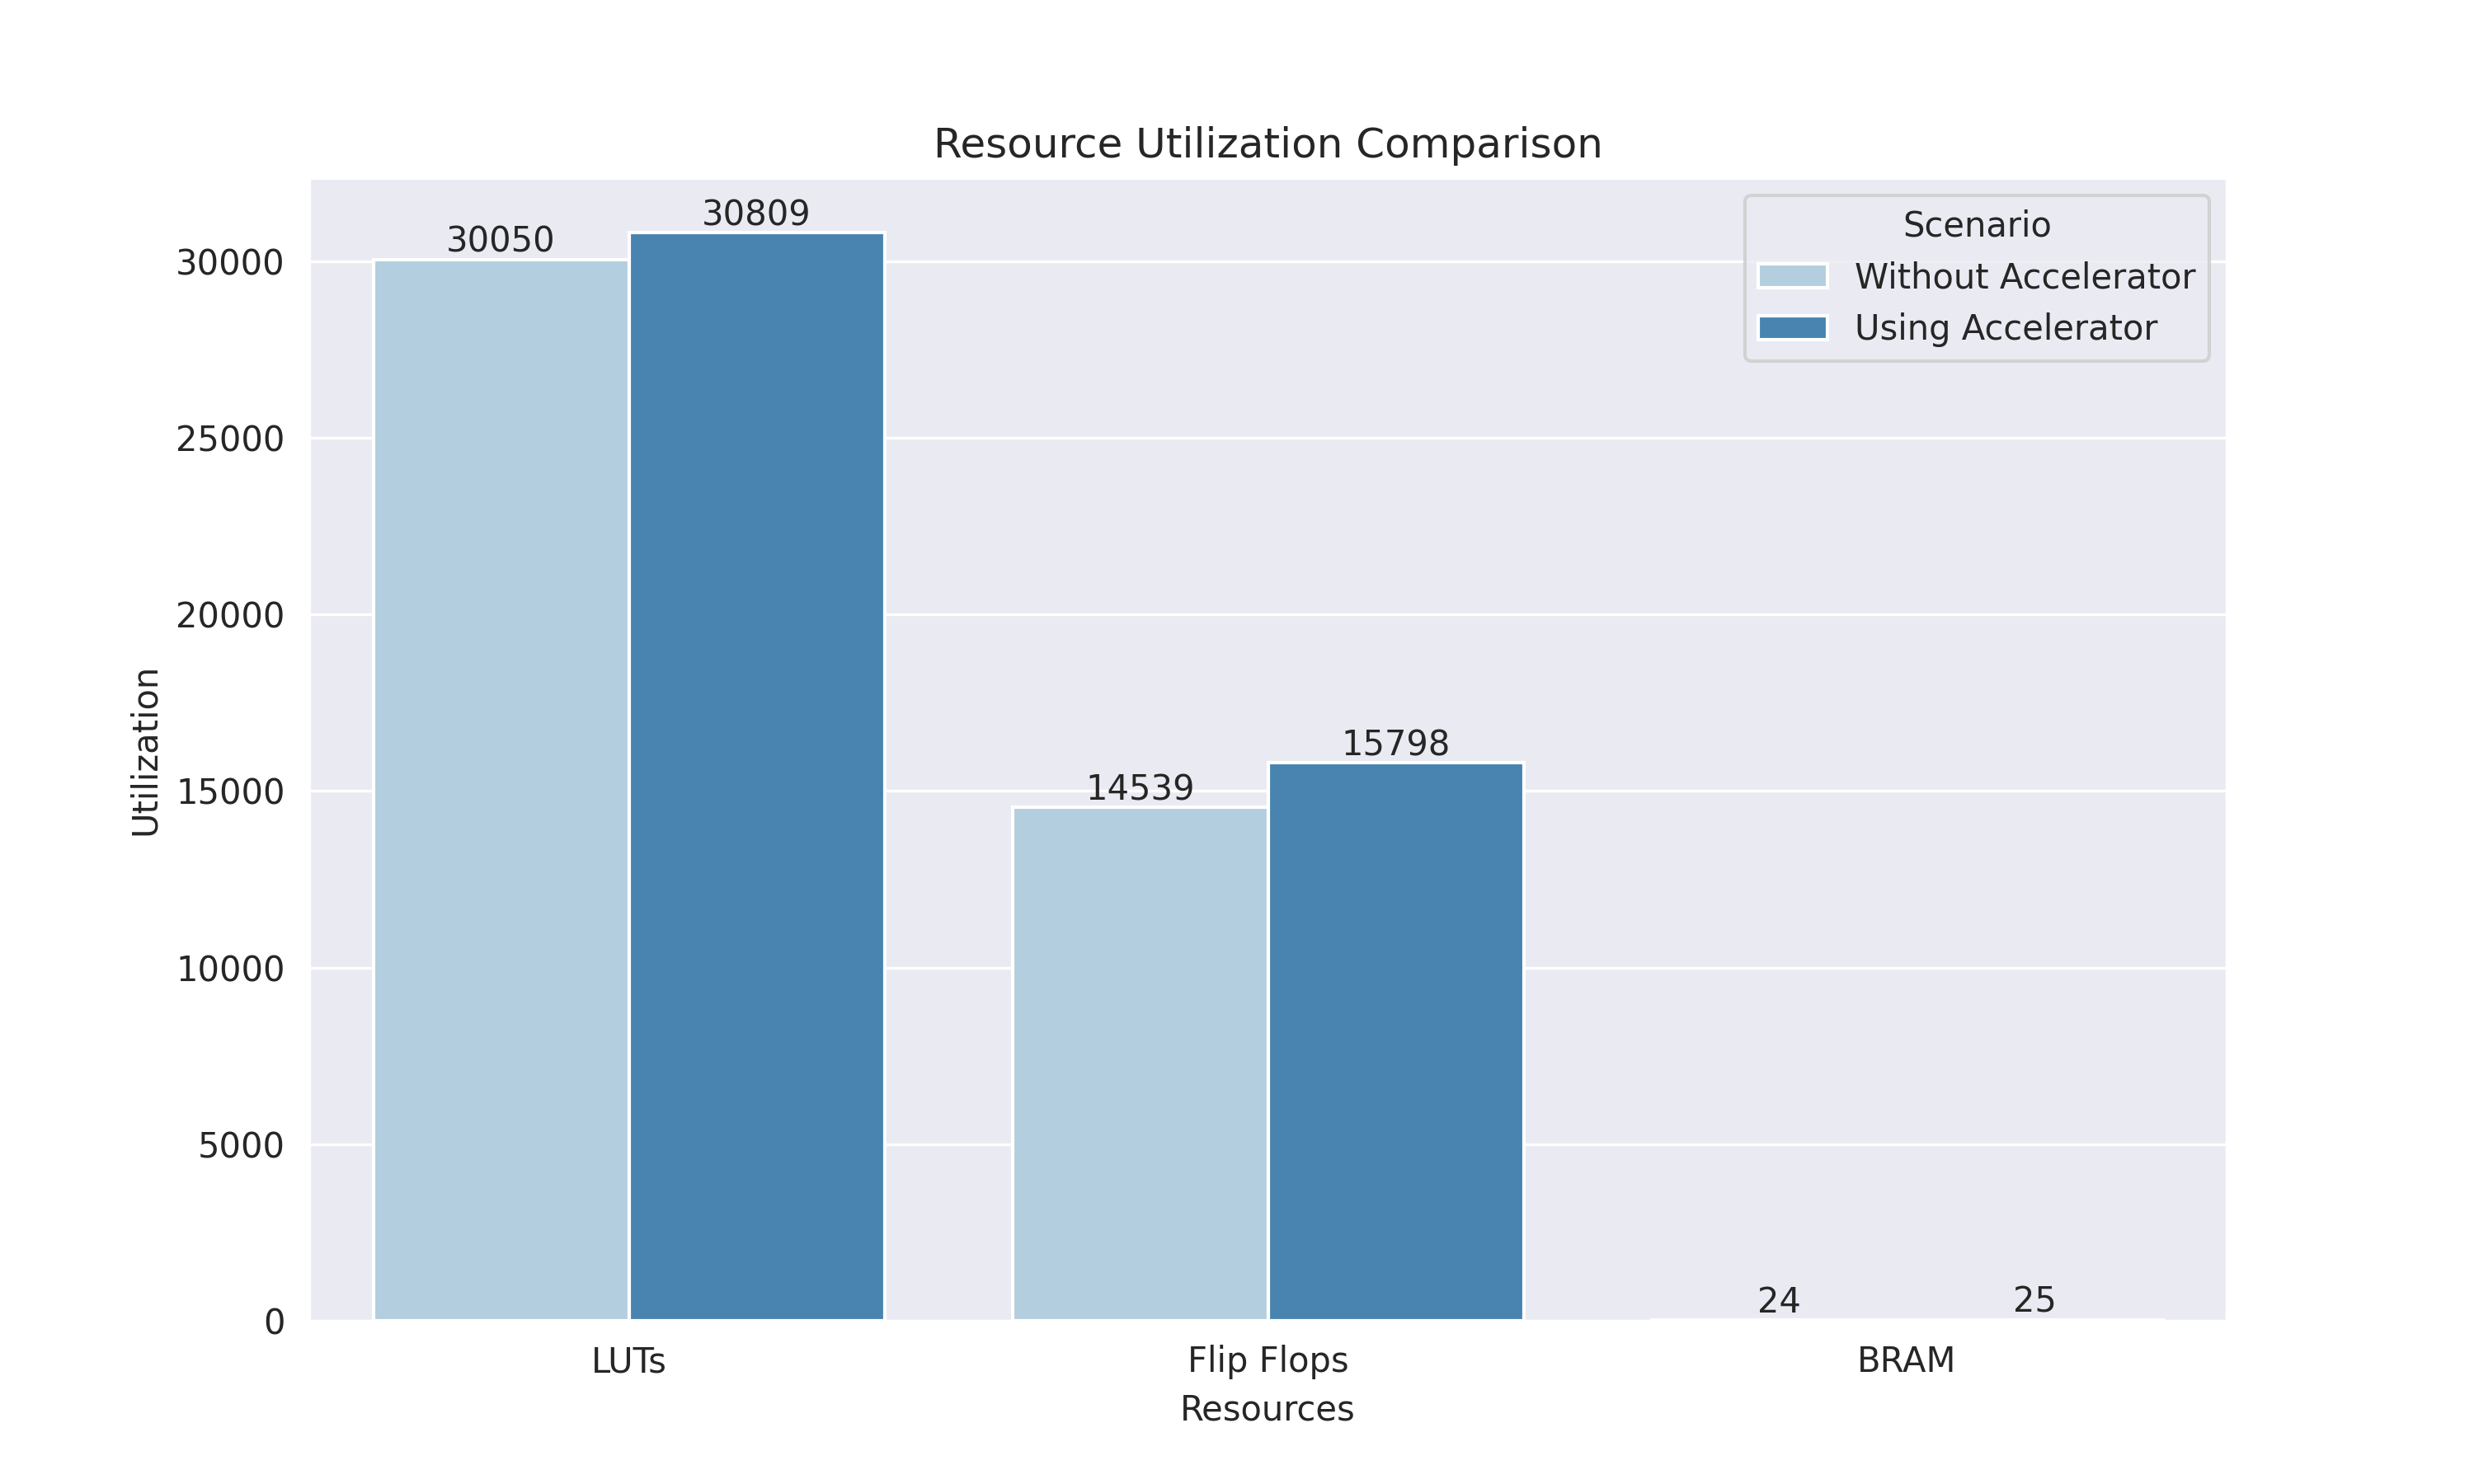
\includegraphics[width=1\textwidth]{chapter-4/plot-resource.png}
	\caption{Plot hasil penggunaan sumber daya pada \ac{FPGA}}
	\label{fig:plot-resource}
\end{figure}

Dapat diperhatikan pada gambar \ref{fig:plot-resource}, perubahan banyaknya penggunaan \ac{LUTs}, \textit{flip-flops}, dan \textit{block \ac{RAM}} itu relatif sedikit. Lebih jelasnya lagi, gambar \ref{fig:plot-resource-increase} mendeskripsikan tentang kenaikan persentase penggunaan sumber daya tersebut beserta dengan banyaknya sumber daya yang masih tersisa pada \ac{FPGA}.

\begin{figure}[h]
	\centering
	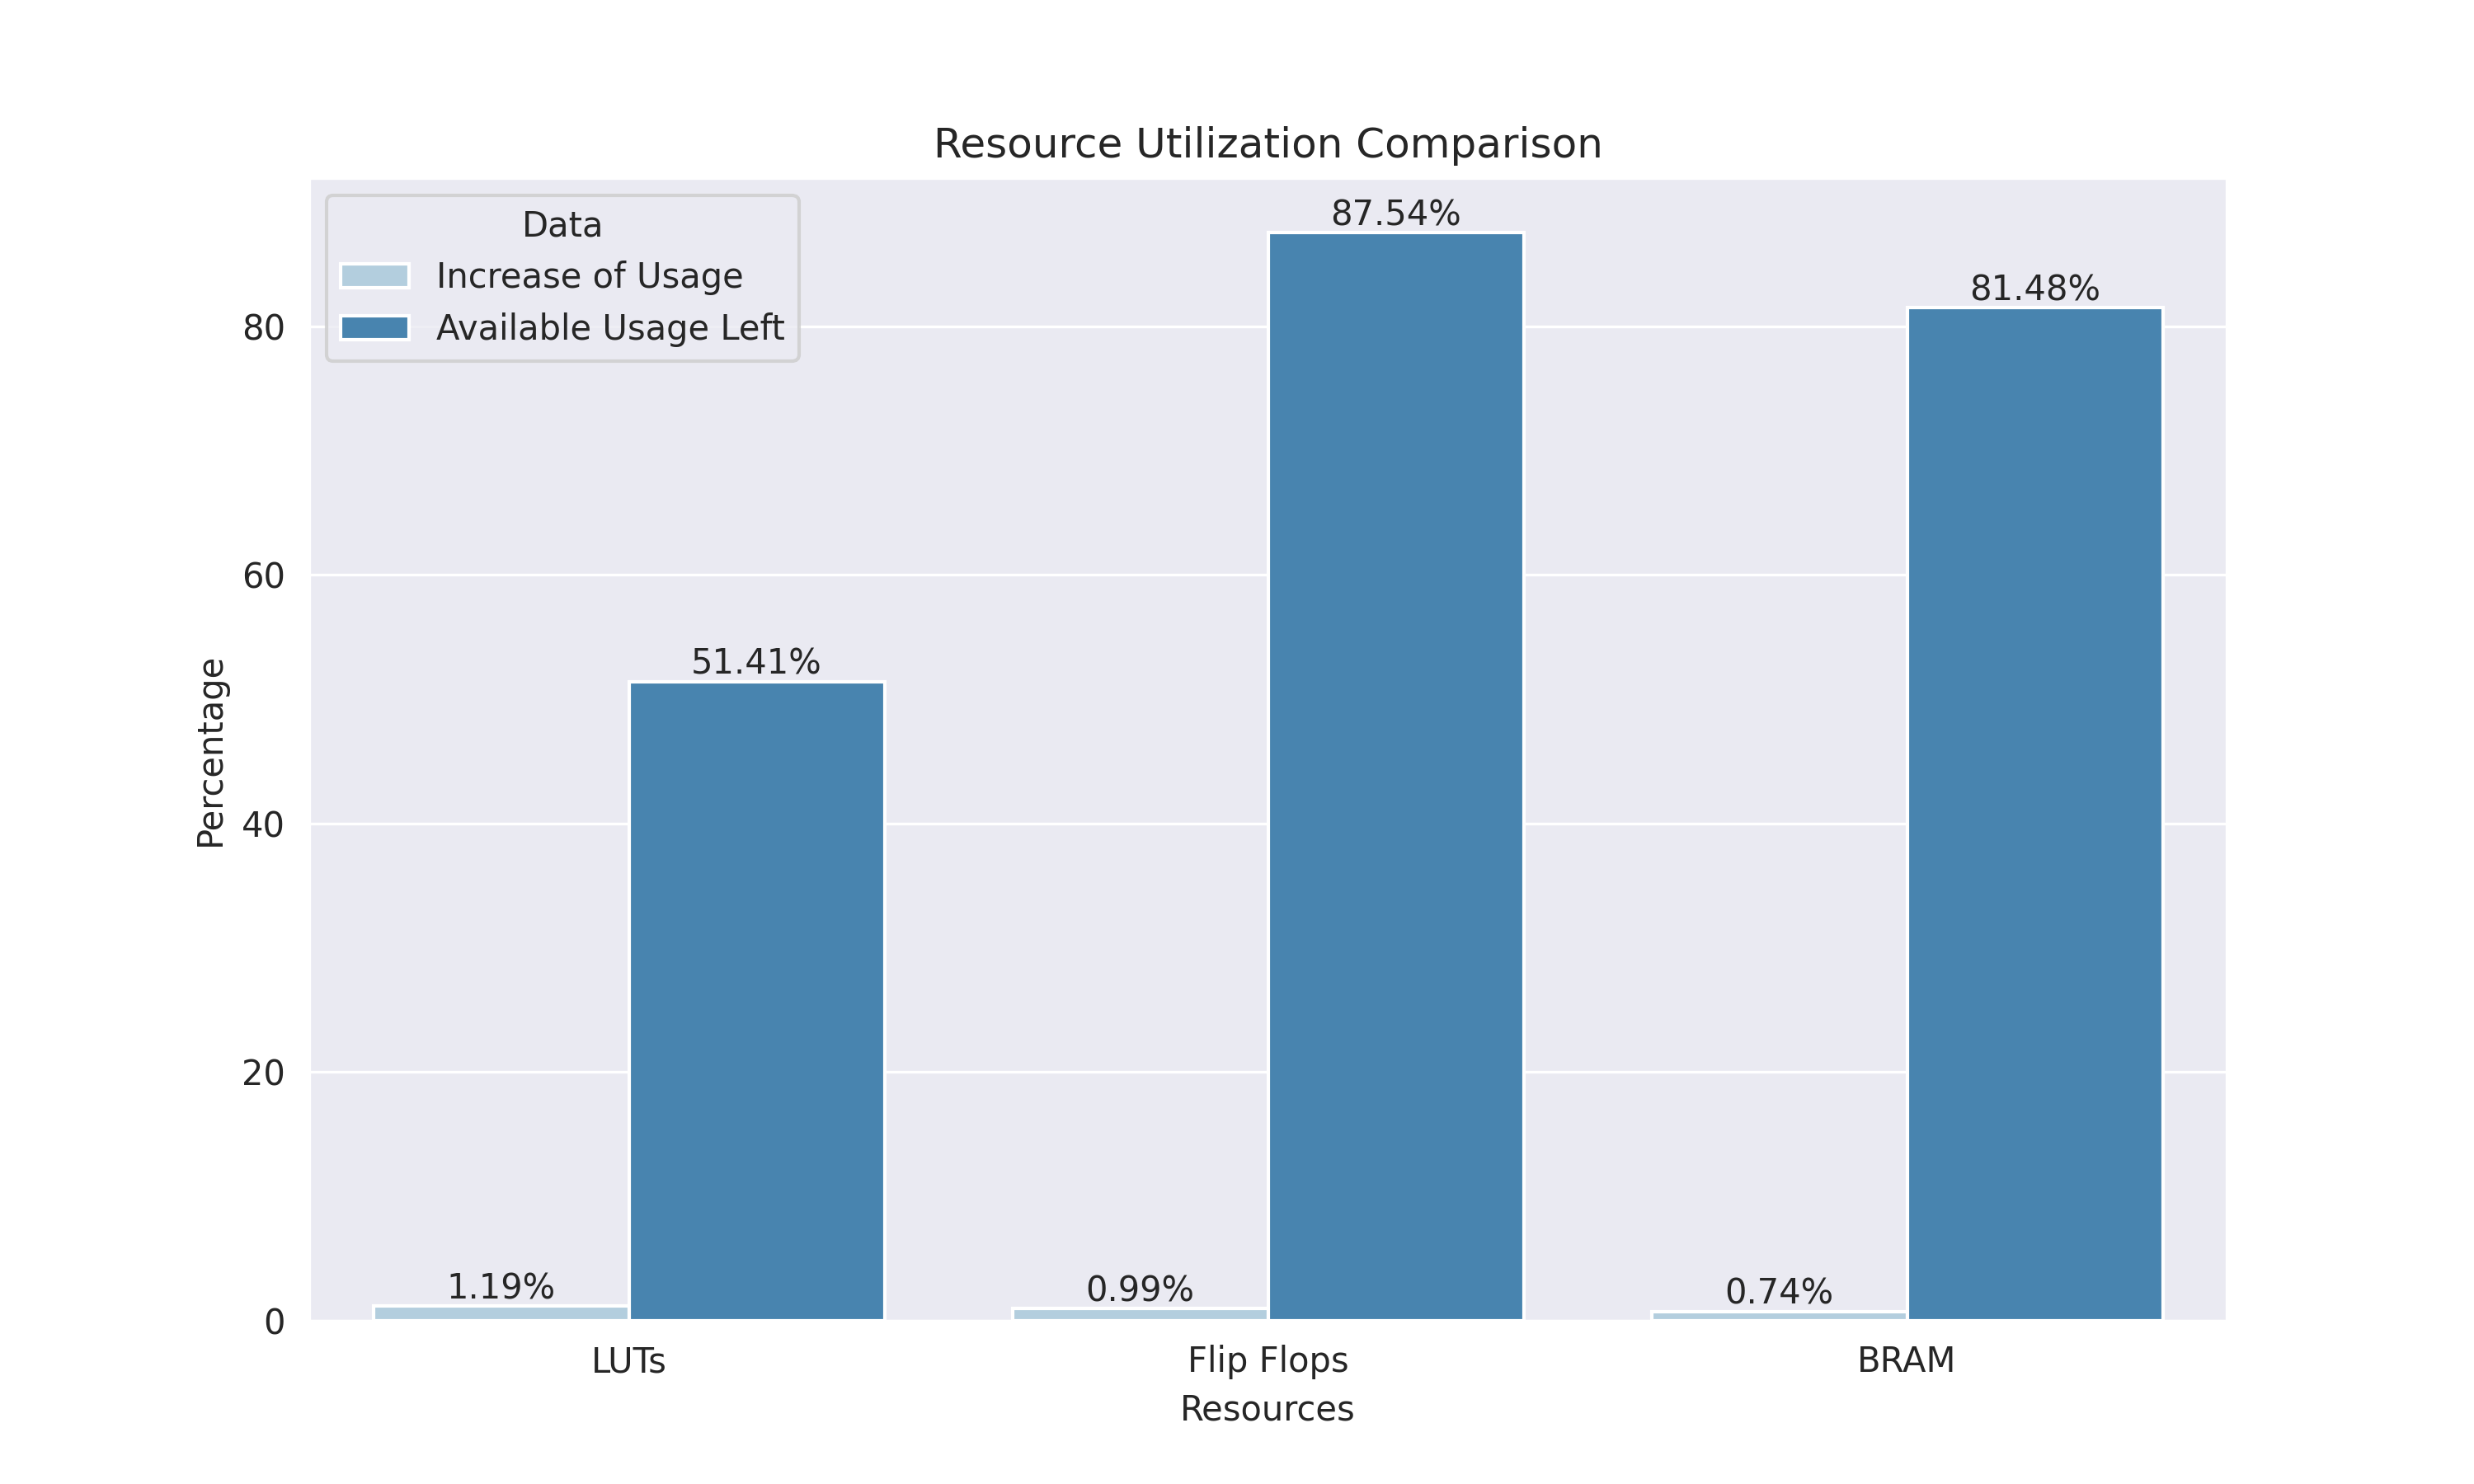
\includegraphics[width=1\textwidth]{chapter-4/plot-resource-increase.png}
	\caption{Plot penambahan penggunaan sumber daya pada \ac{FPGA}}
	\label{fig:plot-resource-increase}
\end{figure}

Seluruh peningkatan sumber daya masih berada dibawah 1.5\% dengan sisa sumber daya tersedia yang masih sangatlah banyak, berarti implementasi akselerator perangkat keras berhasil dibangun secara efisien. Selanjutnya, bila dibandingkan dengan implementasi akselerator-akselerator penelitian sebelumnya yang terdapat pada subbab \ref{sec:accelerator-researches} maka didapatkan data sesuai dengan tabel \ref{tab:comparison-utilization}.


\begin{table}[h]
	\centering
	\caption{Perbandingan utilisasi sumber daya dengan akselerator riset sebelumnya}
	\label{tab:comparison-utilization}
	\renewcommand{\arraystretch}{1.2}
	\setlength{\tabcolsep}{3pt}
	\begin{tabularx}{\textwidth}{|p{20mm}|X|X|X|X|X|X|X|}
		\hline
		\textbf{Reference}            & \multicolumn{2}{c|}{Spanò et al. \parencite{spano2019efficient}} & Da Silva et al. \parencite{dasilva2019parallel} & Y. Meng et al. \parencite{meng2020generic} & \multicolumn{2}{c|}{Sutisna et al. \parencite{sutisna2023faraneq}} & Proposed                            \\ \hline
		\textbf{Design Level}         & \multicolumn{4}{c|}{Standalone Core}                             & \multicolumn{3}{c|}{System on Chip}                                                                                                                                                                     \\ \hline
		\textbf{Action Policy}        & \multicolumn{2}{c|}{NA}                                          & random                                          & $\epsilon$-greedy                          & \multicolumn{2}{c|}{decreasing-$\epsilon$}                         & $\epsilon$-greedy                   \\ \hline
		\textbf{Number of Agents (G)} & single                                                           & single                                          & single                                     & double                                                             & single            & single & single \\ \hline
		\textbf{Bit Width}            & 16                                                               & 32                                              & 30                                         & 16                                                                 & 16                & 32     & 32     \\ \hline
		\textbf{LUT}                  & 333                                                              & 682                                             & 77574                                      & 172                                                                & 2490              & 2062   & 759    \\ \hline
		\textbf{Registers}            & 258                                                              & 606                                             & 13175                                      & NA                                                                 & 2348              & 2179   & 1259   \\ \hline
		\textbf{BRAM}                 & NA                                                               & NA                                              & 266                                        & NA                                                                 & 22                & 20     & 1      \\ \hline
	\end{tabularx}
\end{table}

Pada tabel \ref{tab:comparison-utilization}, dapat diperhatikan bahwa implementasi akselerator yang dibangun pada riset ini merupakan akselerator yang terefisien kedua pada ukuran 32-bit. Hal ini, menunjukkan kemungkinan penggunaan akselerator pada tahap produksi karena dapat bersaing dengan \textit{state of the art} dari penelitian terkini.

\section{Performa Kecepatan Akselerator}
\subsection{Performa Pembelajaran \acl{RL}}
\subsection{Performa \textit{Inference} \acl{RL}}


% Bab ini akan menjelaskan proses implementasi dari rancangan solusi yang telah dikaji pada Bab III. Setelah pembahasan terkait implementasi, akan dilanjutkan dengan pemaparan hasil uji terkait implementasi yang telah dibuat.

% \section{Lingkungan}

\textit{Autoscaler} berbasis kontrol fleksibel akan diimplementasikan di lingkungan komputer lokal. Berikut adalah lingkungan perangkat keras dan perangkat lunak secara terperinci.

Implementasi sistem tugas akhir dilakukan dengan mengimplementasikan dengan bantuan beberapa kakas pada bahasa \textit{python}. Sistem akan hidup di luar \textit{kubernetes cluster} dan mengakses Kubernetes beserta \textit{pods}-nya melalui \textit{Kubernetes Client Library} dan \textit{service Elastic search} melalui \textit{web service} yang dapat diakses dari luar \textit{cluster}.

\textit{Autoscaler} berbasis kontrol fleksibel akan berjalan di \textit{cluster} Kubernetes lokal. Adapun spesifikasi dari komputer yang dipakai untuk pengembangan adalah sebagai berikut.
\begin{enumerate}
    \item \textbf{Perangkat Keras}
    
        \begin{enumerate}
            \item CPU: \textit{Apple M1 Chip}
            \item RAM: 16 GB
        \end{enumerate}
    
    \item \textbf{Perangkat Lunak}
        
        \begin{enumerate}
            \item Platform dan Sistem Operasi: Darwin AMD64, MacOS Monterey 12.6
            \item \textit{Containerization}: Docker
            \item \textit{Kubernetes Cluster}:
                \begin{enumerate}
                    \item Kubernetes Client v1.27.1-eks-2f008fe
                    \item Kubernetes Docker Desktop: Kubernetes v1.25.9
                \end{enumerate}
            \item Bahasa: Python 3.9.12
            \item Dependensi Lain:
                \begin{enumerate}
                    \item \textit{Kubernetes Client Library}
                    \item \textit{Pandas, numpy, statsmodels dan pmdarima}
                    \item \textit{Pickle}
                \end{enumerate}
        \end{enumerate}
\end{enumerate}
% 
% \section{Implementasi}

Bagian ini akan menjelaskan tentang implementasi sistem kontrol adaptif secara terperinci.

\subsection{Batasan Implementasi}
Berikut adalah batasan yang ditetapkan dalam melakukan implementasi sistem kontrol adaptif.
\begin{enumerate}
    \item Masih menerapkan sistem \textit{single node} dan \textit{single pod}.
    \item Tidak memperhatikan optimalisasi dari model ARIMA.
    \item Hanya dapat menangani \textit{metrics} yang sudah ditentukan, yaitu \textit{throughput} dari setiap operasi \textit{Elastic Search} serta utilisasi prosesor hingga memori.
    \item Tidak mempertimbangkan besarnya model seiring bertambahnya data.
    \item Komponen \textit{Metrics Fetcher} berjalan di proses lain dan diimplementasikan dalam \textit{script} yang berbeda dikarenakan bahasa Python memiliki kekurangan dalam penanganan \textit{multithreading}.
    \item Pertukaran data antara komponen \textit{Metrics Fetcher} dan \textit{Predictor} melalui stream file.
\end{enumerate}

\subsection{Kakas yang Digunakan}
Dalam melakukan implementasi ini diperlukan beberapa kakas, diantaranya adalah sebagai berikut.
\begin{enumerate}
    \item \textit{Docker}, \textit{Docker Desktop} dan \textit{Docker Desktop Kubernetes} untuk dipakai sebagai \textit{containerization} dan \textit{cluster} kubernetes lokal.
    \item Minikube dipakai sebagai \textit{cluster} kubernetes lokal dengan versi yang lebih baru karena versi \textit{Docker Desktop Kubernetes} hanya memakai yang \textit{stable} dan tidak bisa dipaksa naik versi.
    \item Pandas dan Numpy untuk keperluan \textit{data processing} serta bentuk data untuk dikirimkan ke komponen lain serta model prediksi ARIMA.
    \item \textit{Kubernetes Python Client} untuk mengontrol \textit{cluster} kubernetes melalui kode Python.
    \item \textit{Pickle} untuk menyimpan model ARIMA sehingga persisten meskipun sistem di-\textit{restart}.
    \item \textit{Statsmodels} dan \textit{pmdarima} untuk membangun model ARIMA serta melakukan otomasi pencarian orde atau lebih dikenal sebagai Auto-ARIMA.
\end{enumerate}

% TODO Untuk spesifikasi pods 
% 
% \section{Pengujian}

Bagian ini akan menjelaskan beberapa skenario yang dilakukan untuk menguji \textit{autoscaler} dengan kontrol fleksibel. Pengujian akan dilakukan per komponen lalu dilanjutkan dengan satu sistem penuh. Setiap skenario pengujian akan dijelaskan tujuannya, skenario yang dilakukan, dan hasil pengujian yang didapatkan.

\subsubsection{Komponen \textbf{\textit{Metrics Fetcher}}}
Seperti yang sudah dijelaskan sebelumnya, komponen ini akan menembak permintaan HTTP pada \textit{Node Stats API} (dokumentasi dapat dilihat pada tautan \url{https://www.elastic.co/guide/en/elasticsearch/reference/current/cluster-nodes-stats.html}) yang telah disediakan \textit{Elastic Search}. Komponen ini akan melakukan transformasi bentuk data menjadi lebih sederhana dan sesuai kebutuhan komponen lainnya. Khusus komponen ini, struktur kodenya tidak memakai sistem kelas dan hanya terdapat sebuah fungsi dan beberapa baris perintah untuk melakukan pemanggilan API, transformasi data dan pengiriman ke \textit{stream file}.
%\subsection{Pengujian Komponen \textit{Predictor}}

Pada bagian ini akan dijelaskan tentang tujuan, skenario, hasil, dan analisis dari pengujian komponen \textbf{\textit{Predictor}}.

\subsubsection{Tujuan Pengujian}

Tujuan pengujian ini memastikan komponen \textbf{\textit{Predictor}} dapat berjalan dengan baik dan menghasilkan data yang sesuai dengan ekspektasi.

\subsubsection{Skenario Pengujian}

Pengujian terhadap komponen \textbf{\textit{Predictor}} dilakukan dengan membandingkan hasil prediksi dengan aktual untuk skenario sebagai berikut.
\begin{enumerate}
    \item \textit{Elastic Search} sedang \textit{idle}.
    \item \textit{Elastic Search} sedang digunakan untuk melakukan operasi penambahan data.
    \item \textit{Elastic Search} sedang digunakan untuk melakukan operasi pencarian data.
\end{enumerate}

\subsubsection{Hasil Pengujian dan Analisis}

% \begin{figure}[h]
%     \centering
%     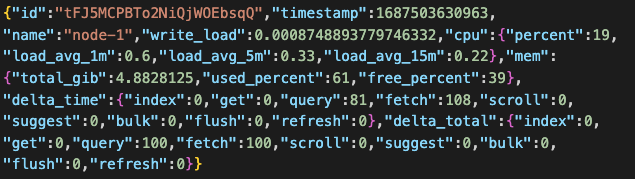
\includegraphics[width=0.8\textwidth]{chapter-4/mf-3.png}
%     \caption{Hasil Pengujian Komponen \textit{Metrics Fetcher} Skenario 3}
%     \label{fig:mf-3}
% \end{figure}

Pengujian komponen \textbf{\textit{Predictor}} menghasilkan angka yang cukup baik sehingga hasil prediksinya bisa dianggap merepresentasikan kondisi aktual.
\subsection{Komponen \textit{Rule Manager}}
Komponen \textbf{\textit{Rule Manager}} berfungsi untuk melakukan parsing terhadap file \textit{rule} yang telah diisi oleh pengguna serta menjadi aggregator untuk melakukan pengecekan \textit{rule} yang berlangsung serta memberi informasi data prediksi kapan saja yang dibutuhkan untuk melakukan pengecekan. Parsing komponen ini menggunakan format csv dan kondisi diekspresikan dengan sintaks python. Komponen akan mengonstruksi objek \textbf{\textit{Rule}} yang akan digunakan oleh komponen \textbf{\textit{Flexible Control}}. Agar terbayang, contoh dari \textit{file rule} dapat dilihat pada gambar \ref{fig:rule-example}. Spesifikasi dari kedua kelas tersebut dapat dilihat pada gambar \ref{fig:rule-spek}.

\begin{figure}[h]
    \centering
    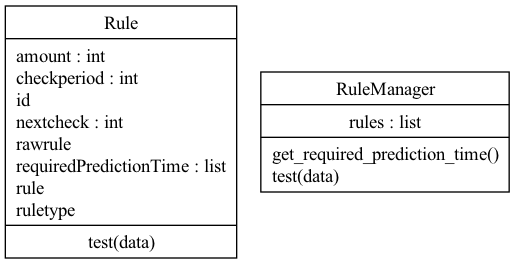
\includegraphics[width=0.8\textwidth]{chapter-4/rule.png}
    \caption{Spesifikasi Kelas Penyusun Komponen \textit{Rule Manager}}
    \label{fig:rule-spek}
\end{figure}

\begin{figure}[h]
    \centering
    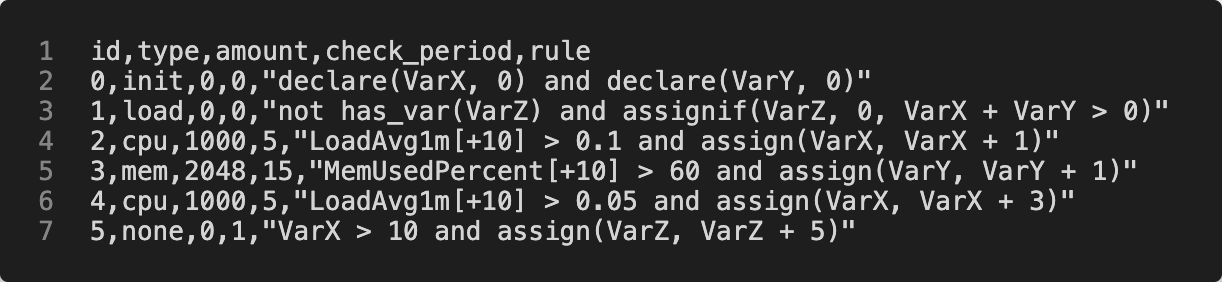
\includegraphics[width=0.75\textwidth]{chapter-4/cth-rule.png}
    \caption{Contoh \textit{File Rule}}
    \label{fig:rule-example}
\end{figure}

Sebuah \textit{rule} memiliki fungsi sebagai berikut.
\begin{enumerate}
    \item Memiliki sebuah kondisi yang akan dievaluasi dengan data prediksi pada waktu prediksi yang diinginkan. Contoh: kondisi \textit{throughput} untuk operasi X untuk 1 menit kedepan dan 5 menit kedepan lebih dari 1s, maka tingkatkan prosesor sebanyak 500m.
    \item Memiliki jumlah serta target kategori untuk diubah, dalam kasus ini pilihannya memori atau prosesor.
    \item Satuan untuk perubahan memori adalah dalam \textit{Mebibyte} atau MiB. Sedangkan untuk prosesor dalam satuan mili atau m.
    \item Sebuah \textit{rule} memiliki periode pengecekan sehingga tidak akan dicek secara terus menerus yang menyebabkan perubahan alokasi sumber daya terlalu cepat. Periode pengecekan dibuat dalam satuan sekon.
\end{enumerate}

Seperti yang bisa dilihat pada contoh gambar \ref{fig:rule-example}, untuk membuat sebuah \textit{rule}, terdapat 5 buah \textit{field} yang harus diisi. \textit{Field} tersebut adalah sebagai berikut.
\begin{enumerate}
    \item \textbf{ID}

        \textit{Field} ini dibebaskan kepada pengguna dan bertipe \textit{string} dan akan digunakan untuk mengidentifikasi \textit{rule} yang dibuat terutama jika terjadi error.
    \item \textbf{\textit{Type}}
    
        \textit{Field} ini bertipe \textit{string} dan akan digunakan untuk mengidentifikasi tipe eksekusi \textit{rule}. Berikut adalah pilihan yang dapat digunakan.
        \begin{enumerate}
            \item \textbf{\textit{Init}}
            
                \textit{Rule} akan otomatis berjalan diawal saat inisiasi (saat pertama kali dijalankan ataupun setelah di-\textit{reset}). Kategori pilihan ini digunakan untuk mendeklarasikan variabel \textit{user-defined} yang bisa digunakan untuk kondisi kompleks atau \textit{rule} yang saling berkaitan.

            \item \textbf{\textit{Load}}
            
                Berbeda dengan inisiasi, \textit{rule} ini akan berjalan ketika sistem dinyalakan dalam kondisi melanjutkan atau sesudah \textit{restart}. Kategori pilihan ini digunakan untuk mendeklarasikan variabel \textit{user-defined} yang mungkin ditambahkan saat \textit{restart}. Pada contoh gambar \ref{fig:rule-example}, dideklarasikan variabel $VarZ$ apabila belum terdefinisi dan $VarX+VarY > 0$.

            \item \textbf{\textit{None}}
            
                \textit{Rule} ini akan berjalan secara periodik namun tidak mengubah alokasi sumber daya apapun. Dapat digunakan untuk melakukan \textit{update} terhadap variabel \textit{user-defined}.

            \item \textbf{\textit{CPU}}

                Seperti namanya, digunakan untuk mengubah alokasi prosesor jika kondisi terpenuhi.
            \item \textbf{\textit{Mem}}
            
            Seperti namanya, digunakan untuk mengubah alokasi memori jika kondisi terpenuhi.
        \end{enumerate}

    \item \textbf{\textit{Amount}}
    
        \textit{Field} ini hanya berguna apabila tipe \textit{rule} adalah \textbf{CPU} atau \textbf{Mem}. Seperti namanya, digunakan untuk mengatur jumlah perubahan. Untuk \textbf{CPU}, angka dalam satuan milli. Sedangkan, untuk \textbf{Mem}, angka dalam satuan \textit{Mebibyte} (MiB).
    
    \item \textbf{\textit{Check Period}}
        
        \textit{Field} ini digunakan untuk mengatur periode pengecekan dalam satuan sekon. Periode ini berfungsi sebagai \textit{cooldown} jika kondisi bernilai benar. Setiap \textit{rule} yang ada akan dicek secara global setiap sekon, namun jika sudah bernilai benar, akan memasuki periode tidak dicek sampai periode pengecekan selesai. Jika kondisi bernilai salah, maka akan dicek kembali pada detik berikutnya. Tidak berlaku untuk tipe \textbf{init} dan \textbf{load} karena dua tipe tersebut akan selalu dijalankan sekali pada saat inisiasi atau \textit{restart}.

    \item \textbf{\textit{Rule}}
        
        \textit{Field} ini berisikan kondisi yang akan dievaluasi. Kondisi ini harus berupa ekspresi boolean yang terdiri dari variabel \textit{user-defined}, variabel prediksi metrik sistem dan operator logika. Variabel \textit{user-defined} dapat berupa variabel yang dideklarasikan pada \textit{rule} dengan tipe \textbf{init} atau \textbf{load} atau variabel yang dideklarasikan pada \textit{rule} lainnya. Operator logika yang dapat digunakan adalah \textbf{and}, \textbf{or}, dan \textbf{not}. Untuk operator perbandingan yang dapat digunakan adalah \textbf{$==$}, \textbf{$!=$}, \textbf{$>$}, \textbf{$>=$}, \textbf{$<$}, dan \textbf{$<=$}. Untuk operator aritmatika yang dapat digunakan adalah \textbf{+}, \textbf{-}, \textbf{*}, \textbf{/}, dan \textbf{\%}.

        Terdapat batasan berupa tidak bisa meletakkan variabel prediksi metrik sistem pada \textit{rule} bertipe \textbf{init} dan \textbf{load}. Apabila ingin menggunakan variabel prediksi metrik sistem, maka harus menggunakan tipe \textbf{CPU} atau \textbf{Mem}.

        Untuk variabel \textit{user-defined}, batasan yang ada adalah penamaan variabel harus dilakukan layaknya \textit{script} pada umumnya, seperti tidak bisa dimulai dengan angka, namun bisa diakhiri oleh angka dan tidak boleh mengandung simbol selain garis bawah.

        Sedangkan, untuk variabel metrik sistem yang dapat digunakan adalah sebagai berikut.

        \begin{enumerate}
            \item \textbf{\textit{Write Load}}
            \item \textbf{\textit{Index}}\label{item:index}
            \item \textbf{\textit{Get}}
            \item \textbf{\textit{Query}}
            \item \textbf{\textit{Fetch}}
            \item \textbf{\textit{Scroll}}
            \item \textbf{\textit{Suggest}}
            \item \textbf{\textit{Bulk}}
            \item \textbf{\textit{Flush}}
            \item \textbf{\textit{Refresh}}\label{item:refresh}
            \item \textbf{\textit{CPUPercent}}\label{item:cpupercent}
            \item \textbf{\textit{LoadAvg1m}}\label{item:load-avg-1}
            \item \textbf{\textit{LoadAvg5m}}
            \item \textbf{\textit{LoadAvg15m}}\label{item:load-avg-15}
            \item \textbf{\textit{MemUsedPercent}}\label{item:mempercent}
        \end{enumerate}

        Untuk nomor \ref{item:index} sampai \ref{item:refresh} adalah \textit{throughput} operasi-operasi \textit{Elastic Search} dalam bentuk milisekon. Sedangkan, \ref{item:cpupercent} dan \ref{item:mempercent} adalah pemakaian CPU dan memori dalam bentuk bilangan bulat 1-100 yang merepresentasikan persen pemakaian. \textit{Load Average} adalah indikator beban sistem dalam 1, 5, dan 15 menit terakhir. Biasanya angka ini digunakan untuk menentukan turun naiknya beban prosesor sistem. Apabila menunjukkan kenaikan, maka dapat dipastikan bahwa sistem mulai digunakan. Sedangkan, apabila menunjukkan penurunan, maka sistem mulai tidak digunakan. Persamaan \ref{eq:load-average} akan digunakan untuk menjelaskan angka pada \textit{Load Average}. Pada persamaan tersebut, $U(t)$ adalah persen utilisasi di waktu $t$. Sebagai contoh, ketika $LoadAvg(t)$ bernilai $1.0$ dan $NumberOfCPU$ adalah $4$, maka dapat disimpulkan bahwa persentase utilisasi CPU adalah $25\%$ sehingga bisa disimpulkan sebagai sistem belum maksimal dimanfaatkan. Namun, variabel ini biasanya bercampur juga dengan utilisasi prosesor dari sistem, jaringan, file I/O dan network I/O berbeda dengan \textit{CPUPercent} yang murni menunjukkan utilisasi prosesor dari sistem untuk proses \textit{Elastic Search}.

        \begin{equation}
            \label{eq:load-average}
            U(t) = LoadAvg(t)/NumberOfCPU*100
        \end{equation}
\end{enumerate}
\subsection{Komponen \textit{Resource Controller}}

Seperti yang sudah dirancangkan sebelumnya, kelas ini menggunakan \textit{Kubernetes Client API} untuk mengubah alokasi sumber daya. Diimplementasikan dengan sistem antrian, sehingga jika sejumlah rule aktif secara bersamaan, maka akan dijalankan secara berurutan. Terdapat sebuah fungsi \textit{tick} yang akan berfungsi untuk mengeksekusi antrian. Contoh simpanan file antrian dapat dilihat pada gambar \ref{fig:ex-queue-rc}. File tersebut menyimpan status alokasi sumber daya pada saat itu, kapan melakukan perubahan pada antrian berikutnya dalam waktu UNIX dan antrian yang akan dieksekusi satu per satu.

\begin{figure}[h]
    \centering
    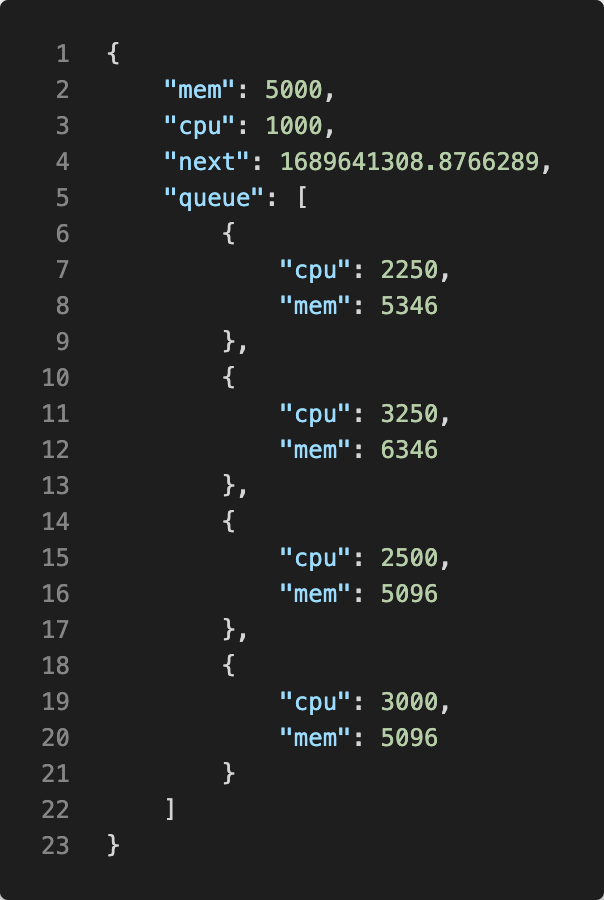
\includegraphics[width=0.45\textwidth]{chapter-4/rc-queue-ex.png}
    \caption{Contoh File Antrian Pengubahan Alokasi}
    \label{fig:ex-queue-rc}
\end{figure}

% TODO CONTOH SISTEM ANTRIAN
\subsection{Komponen \textit{Flexible Control}}

\textbf{\textit{Flexible Control}} mengkolaborasikan \textbf{\textit{Rule Manager}}, \textbf{\textit{Resource Controller}}, \textbf{\textit{Predict Component Factory}} dan \textbf{\textit{Predict Component Storage}}. Komponen ini akan meminta list waktu prediksi yang diperlukan dari \textbf{\textit{Rule Manager}} untuk \textbf{\textit{Rule Manager}} sehingga \textbf{\textit{Predict Component Storage}} dapat menyediakan data prediksi. Setelah itu, semua \textbf{\textit{Rule}} yang memenuhi syarat akan langsung ditransformasikan dan dikirim ke komponen \textbf{\textit{Resource Controller}}. Selain itu, komponen ini juga bertanggung jawab meneruskan data ke \textbf{\textit{Predict Component Storage}} untuk melakukan penambahan data. Spesifikasi kelas ini dapat dilihat pada gambar \ref{fig:ac-spek}.

\begin{figure}[h]
    \centering
    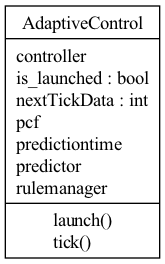
\includegraphics[width=0.3\textwidth]{chapter-4/ac.png}
    \caption{Spesifikasi Kelas Penyusun Komponen \textit{Flexible Control}}
    \label{fig:ac-spek}
\end{figure}

% \subsection{Pengujian X}

% \subsubsection{Tujuan Pengujian}

% \subsubsection{Skenario Pengujian}

% \subsubsection{Hasil Pengujian dan Analisis}
% 
% \section{Perbandingan}

Bagian ini akan menjelaskan pengujian dampak dari \textit{autoscaler} dengan kontrol fleksibel. Pengujian akan dilakukan dengan membandingkan \textit{autoscaler} yang dibuat dengan sistem kontrol fleksibel dengan \textit{autoscaler} sederhana yang memakai \textit{treshold} serta tanpa \textit{autoscaler}. 

% \subsection{Perbandingan Performa}

\subsection{Perbandingan Efisiensi}

Bagian ini akan menjelaskan perbandingan \textit{autoscaler} antara metode yang diimplementasikan dengan metode yang disediakan kubernetes.

\subsubsection{\textit{Horizontal Pod Autoscaler}}

Metode ini melakukan replikasi terhadap \textit{pods} dengan menambah \textit{pods} baru apabila utilisasi sumber daya melewati suatu ambang batas. Sebagai informasi, agar \textit{Elastic Search} dapat berjalan dengan normal dibutuhkan memori minimal 4 GB. Sedangkan, dalam aplikasi skala yang kecil, akan kurang efisien apabila diperlukan 4 GB untuk setiap \textit{pods} ketika dibutuhkan hanya penambahan 2GB memori. Ditambah, penambahan sumber daya memori menjadi minimal kelipatan 4GB. Sehingga, dalam kasus ini, implementasi kontrol fleksibel lebih bebas mengatur dibandingkan dengan \textit{Horizontal Pod Autoscaler}.

\subsubsection{\textit{Vertical Pod Autoscaler}}

Seperti yang sudah dijelaskan pada studi literatur, metode ini biasanya digunakan untuk memperbanyak alokasi sumber daya jika pemakaian sudah melewati ambang batas tertentu. Namun, ternyata setelah diteliti lebih lanjut, metode ini tidak bisa dilakukan oleh Kubernetes pada aplikasi yang berbasis JVM. \textit{Vertical Pod Autoscaling} belum siap digunakan dengan aplikasi berbasis JVM karena keterbatasan Kubernetes dalam melihat penggunaan memori yang sebenarnya, \parencite{googlevpajvm}. Hal ini tentu masuk akal karena JVM langsung mengambil memori sepenuhnya yang dialokasikan, untuk melihat pemakaian yang sesungguhnya, harus melihat dari dalam aplikasi tersebut. Oleh karena itu, secara tidak langsung, metode menarik metrik penggunaan memori dari dalam \textit{Elastic Search} yang diimplementasikan menjadi salah satu keunggulan sistem yang diimplementasikan.
